\section{Классификация БАС}

Единой классификации нет — БАС делят по нескольким признакам. На экзамене обычно спрашивают: по \textbf{схеме (типу)}, по \textbf{массе}, по \textbf{дальности / радиусу}, по \textbf{способу управления} и по \textbf{назначению}.

\subsection{По аэродинамической схеме (типу летательного аппарата)}

\begin{figure}[H]\centering
\begin{subfigure}[b]{0.24\linewidth}\centering
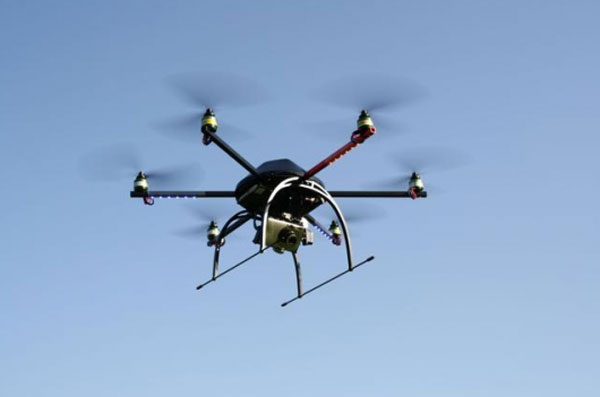
\includegraphics[width=\linewidth,height=30mm,keepaspectratio]{img/hexacopter.jpg}
\caption{Мультироторный}\end{subfigure}\hfill
\begin{subfigure}[b]{0.24\linewidth}\centering
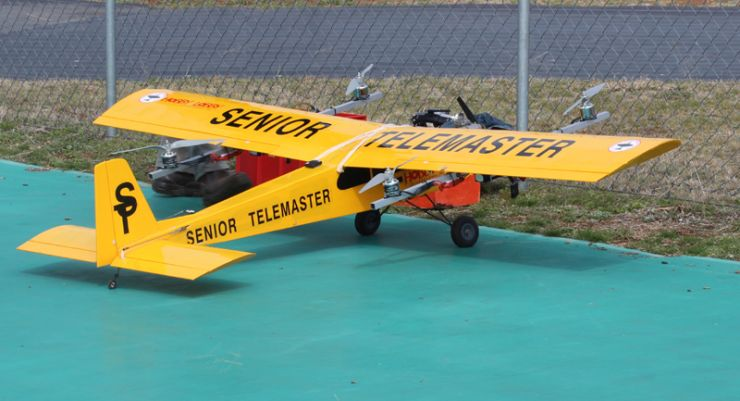
\includegraphics[width=\linewidth,height=30mm,keepaspectratio]{img/vtol.jpg}
\caption{Самолётный}\end{subfigure}\hfill
\begin{subfigure}[b]{0.24\linewidth}\centering
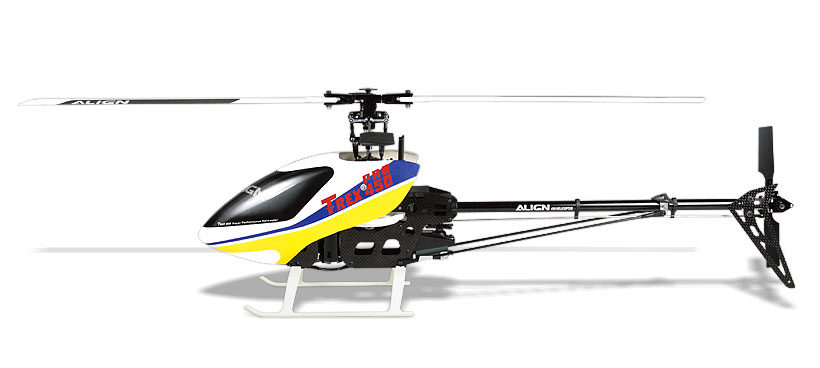
\includegraphics[width=\linewidth,height=30mm,keepaspectratio]{img/heli.jpg}
\caption{Вертолётный}\end{subfigure}\hfill
\begin{subfigure}[b]{0.24\linewidth}\centering
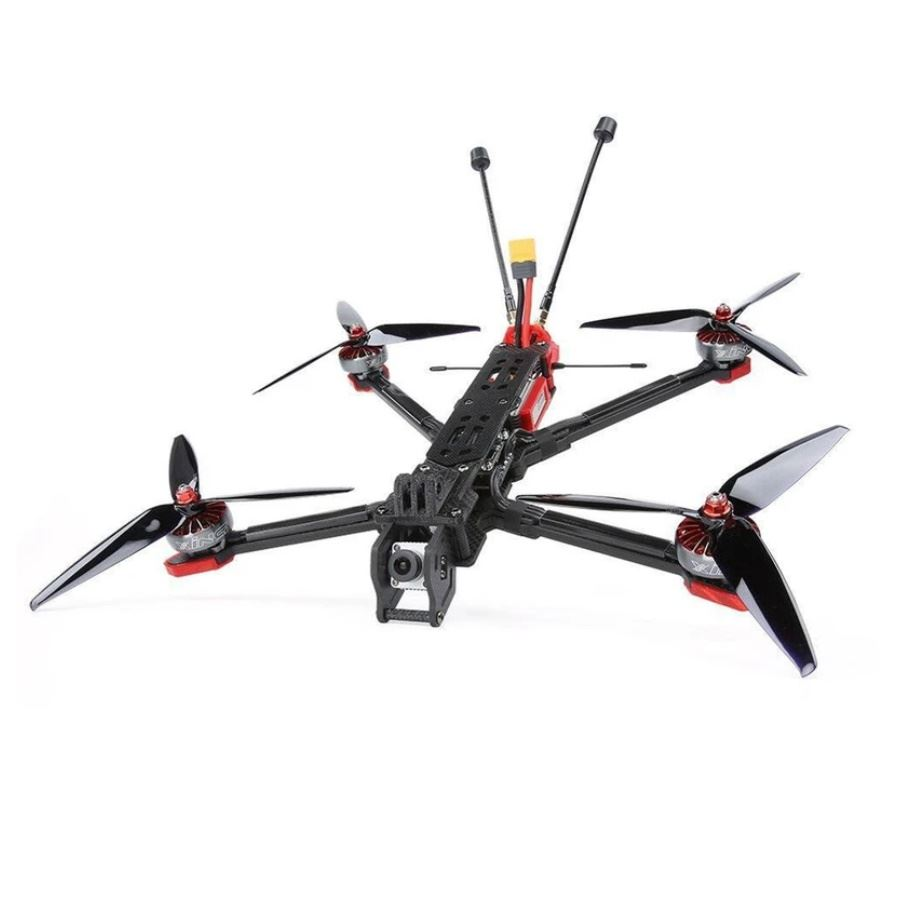
\includegraphics[width=\linewidth,height=30mm,keepaspectratio]{img/fpv-quad.jpg}
\caption{FPV-квадрокоптер}\end{subfigure}
\caption{Основные схемы БВС {\color{gray}\scriptsize(фото: ArduPilot Wiki)}}
\end{figure}

\begin{table}[H]\centering\small
\renewcommand{\arraystretch}{1.3}
\begin{tabularx}{\linewidth}{@{}>{\raggedright\arraybackslash}p{33mm} X X@{}}
\toprule
\textbf{Тип} & \textbf{Плюсы} & \textbf{Минусы} \\
\midrule
\textbf{Мультироторный} (квадро-, гекса-, октокоптер) & Вертикальный взлёт, зависание, простая механика, дешёвый & Малое время полёта (\SIrange{5}{40}{\minute}), низкий КПД \\
\textbf{Самолётного типа} (классика, «летающее крыло») & Большая дальность и время полёта (часы), высокая скорость, экономичность & Нужна площадка/катапульта для взлёта и посадки, не может зависать \\
\textbf{Вертолётного типа} & Зависание, большая грузоподъёмность, один большой ротор эффективнее & Сложная механика (автомат перекоса), сложен в обслуживании \\
\textbf{Гибридный (VTOL)} — конвертоплан, «квадроплан», tail-sitter & Взлёт как коптер, полёт как самолёт & Сложность, лишняя масса моторов в крейсерском полёте \\
\textbf{Аэростатный / привязной} & Очень долгое нахождение в воздухе & Зависимость от ветра, большие размеры \\
\bottomrule
\end{tabularx}
\caption{Сравнение схем}
\end{table}

\subsection{По массе}
\begin{itemize}
\item \textbf{Правовая (РФ)}: до \SI{0.15}{\kilo\gram} — без учёта; \SIrange{0.15}{30}{\kilo\gram} — учёт; более \SI{30}{\kilo\gram} — государственная регистрация (см. раздел 1).
\item \textbf{Техническая (распространённая)}: \emph{нано/микро} — до \SI{0.25}{\kilo\gram} (tiny whoop, DJI Mini); \emph{мини} — до \SIrange{5}{7}{\kilo\gram}; \emph{лёгкие} — до \SI{30}{\kilo\gram}; \emph{средние} — до \SI{150}{\kilo\gram}; \emph{тяжёлые} — более \SI{150}{\kilo\gram}.
\end{itemize}

\subsection{По дальности (радиусу действия) и высоте}
\begin{table}[H]\centering\small
\begin{tabularx}{\linewidth}{@{}l >{\raggedright\arraybackslash}X >{\raggedright\arraybackslash}X@{}}
\toprule
\textbf{Класс} & \textbf{Радиус} & \textbf{Пример} \\
\midrule
Ближнего действия (Close Range) & до \SIrange{10}{30}{\kilo\metre} & FPV-дроны, DJI Mavic, «Геоскан 201» \\
Малой дальности (Short Range) & \SIrange{30}{70}{\kilo\metre} & «Орлан-10»\\
Средней дальности (Medium Range) & \SIrange{70}{200}{\kilo\metre} & — \\
MALE (Medium Altitude Long Endurance) & сотни км, высота до \SI{9}{\kilo\metre}, 24+ ч & «Орион», MQ-1 \\
HALE (High Altitude Long Endurance) & тысячи км, высота до \SI{20}{\kilo\metre} & RQ-4 Global Hawk \\
\bottomrule
\end{tabularx}
\caption{Классификация по дальности (по UVS International)}
\end{table}

\subsection{По способу управления}
\begin{itemize}
\item \term{Ручное (дистанционно пилотируемое)} — пилот управляет в реальном времени: по прямой видимости (LOS) или по видео (\term{FPV}, First Person View — «вид от первого лица»).
\item \term{Автоматическое} — полёт по заранее заданной программе (миссии по точкам GPS), пилот контролирует и может вмешаться.
\item \term{Автономное} — БВС сам принимает решения (обход препятствий, распознавание целей, навигация без GNSS).
\end{itemize}

\subsection{По назначению}
Гражданские (аэрофотосъёмка, картография, мониторинг ЛЭП и трубопроводов, сельское хозяйство — опрыскиватели, доставка, МЧС, спорт/FPV-гонки, кино), государственные (полиция, пограничники), военные (разведка, корректировка, ударные). \par
Для FPV-дронов отдельно используют \textbf{классификацию по размеру пропеллера}: \emph{whoop} 1–2" (\SIrange{65}{85}{\milli\metre}), \emph{cinewhoop} 2,5–3,5" (с защитой пропеллеров), \emph{freestyle/racing} 5", \emph{long range} 7", \emph{heavy} 8–10"+.

\begin{exam}
\begin{enumerate}
\item Назовите преимущества и недостатки мультироторной и самолётной схем.
\item Что такое VTOL и зачем он нужен?
\item Чем автоматическое управление отличается от автономного?
\end{enumerate}
\end{exam}
